\section{Evaluation of the system in general}

The previous section presented the system that is NUIssues, relevant models, and planning behind the system. This section evaluates the prototype by looking at \textcite[34]{wigdow-wixon:brave-nui-world:2011}'s guidelines for 2D spatial NUI design on how to support using 2D planar space, and some valuable outcomes and actionable events.

\subsection{NUI guidelines}

The only mandatory guideline for spatial 2D NUI design in \textcite[34]{wigdow-wixon:brave-nui-world:2011} is that the design must:

\begin{quote}
"Create an environment that is optimized for touch in its layout, feedback, metaphors, and behaviors. Any item that responds to users' touch must be at least 15mm in size in all directions, and there must be at least 5 mm between minimally sized touch targets".
\end{quote}

NUIssues is true to this: on the target device, all \textit{cards} have more than 5 mm margin to the next card, and each card is (much) more than 15 mm in all directions. This is demonstrated in \ref{figure:standard-view}.

\begin{figure}[H]
    \centerline{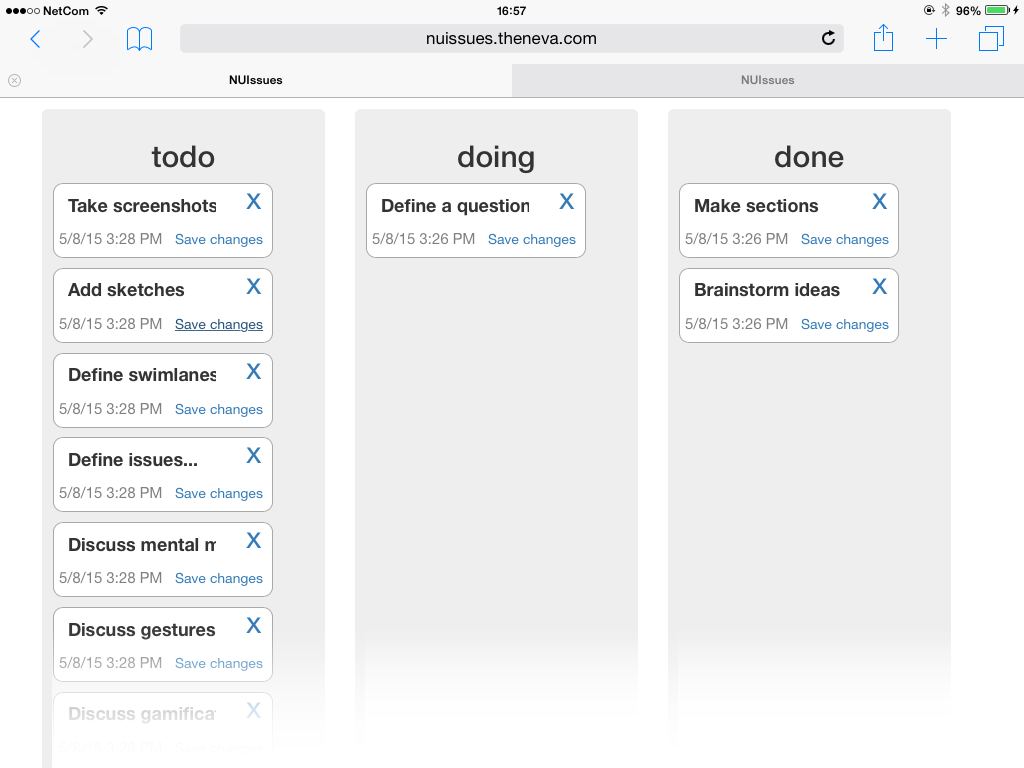
\includegraphics[scale=0.4]{images/nuissues-screenshots/01-default-all-swimlanes}}
    \caption{Standard view of NUIssues with issues in all swimlanes}
    \label{figure:standard-view}
\end{figure}

A key concern here is scrolling within a swimlane, which is not hinted at in any way other than blank space to the right of the cards inside the swimlans. While more content is hinted at through a fading swimlane, only users familiar with touch interfaces with scrolling may possibly understand how to manipulate this list. This weakness is a substantial flaw in the design that should be revised in future iterations of the design.

The following points are \textit{guidelines}, listed under "Should" in \textcite[34]{wigdow-wixon:brave-nui-world:2011}.

The design is consistent through the application, and the user is not allowed to customise the look of the app because the entire interface only consists of one single view.

The spatial relationships of the issues have been considered:

\begin{itemize}
  \item In the Western world, we read from left to right, and thus the natural lifecycle of a card moves from left (\textit{todo}) to right, ultimately reaching \textit{done}.
  \item While not explicitly expressed in the design (so that the user is left to interpret the significance of the positioning), one may assume that the user's model of the system identifies issues higher up (with a lower index) as more urgent or important. After all, the grid layout imposes a hierachical style on the application. This interpretation is, however, intentionally left to the user. 
\end{itemize}

NUIssues is not designed to be a multi-user system, although changs one user makes to the board affect every user of the same instance. Multitouch support would be interesting, but counter-intuitive in an application specifically designed for a personal tablet computer.

The main (and only) view has only the minimally required controls at any given time, and focuses on the \textit{content} of the application -- as does the user.

Finally, direct manipulation has been actively considered: manipulation always happens inline (only the title in the prototype), with no external prompts except the virtual keyboard on the tablet unless a physical keyboard is connected -- which cannot be avoided.

Each card can be deleted individually, and accidental occlusion is prevented by highlighting the entire card if it is about to be deleted. One thing to note is that \textit{only} using colour is not necessarily enough to indicate a status.

\subsection{Potential sources of errors}

There are several potential sources of error in a touch application. One of the most important, \textit{fat fingers} as defined by \textcite[73]{wigdow-wixon:brave-nui-world:2011} have been avoided to an extent by spacing and sizing elements in compliance with guidelines for 2D NUI design.

Other error sources include multiple capture states, accidental activation (like brushing the screen with an arm), physical manipulation constraints, stolen capture, and tabletop debris, which are all very difficult to counter with no real control over the actual use or environment for using the application.

\subsection{Other notes and models}

All objects on screen (except \textit{swimlanes}) are interactive (editable, draggable, or sortable) through touch. Landing a finger on a card allows the user to drag the card to another position by sliding onto the closest new position and release the card to the new position by lifting the finger off the card. Landing a finger specifically on an editable text area on the card (the title) and immediately lifting the finger off, then editing the text with help of a keyboard. In this case a \textit{gesture} \parencite[157]{wigdow-wixon:brave-nui-world:2011} as an exit sequence would be helpful, but this is not implemented in the prototype.

While the application does not support any gestures, looking at Piaget's concept of the INRC group \parencite[137]{wigdow-wixon:brave-nui-world:2011}. This group defines four properties:

\begin{itemize}
  \item Identity, stating that performing equivalent actions (like moving an issue to another swimlane) should reliably do an equivalent action;
  \item Negation, stating that it should be possible to return to the object's previous state after starting an action by performing the opposite action. For example, when dragging a card out of its place, backtracing to where the card was picked up from and releasing the card will invariably return it to its origin.
  \item Reciprocal, stating that there are actions that return some aspect of the system to its original state. This is not implemented in NUIssues, but could take the form of an undo button.
  \item Commutative, stating that changing the order of independent operations does not affect the end result. For example, changing the title of an issue and then moving its card to a different swimlane ultimately results in the same system state as first moving the card and then changing the title of the issue.
\end{itemize}

\subsection{Meaningful graphical states and actionable events}

The entire application only has one single screen, but this view provides information in several different ways. Each state, or "view", will be provided in a screenshot, followed by a brief summary of the meaning of the state.

\begin{figure}[H]
    \centerline{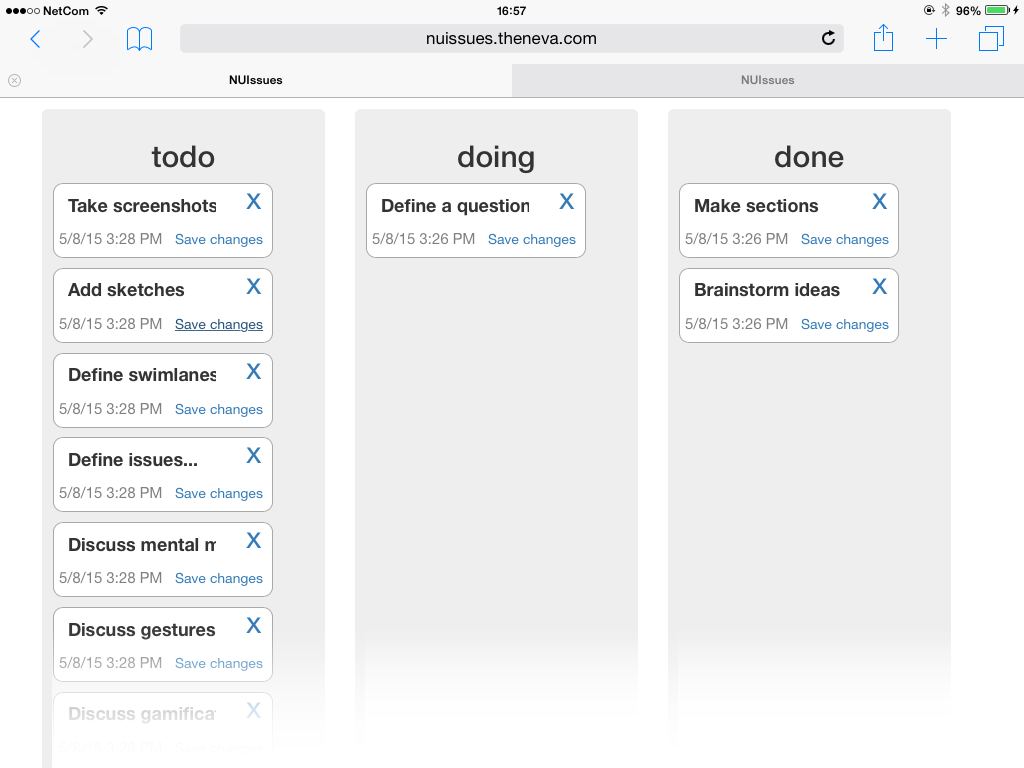
\includegraphics[scale=0.4]{images/nuissues-screenshots/01-default-all-swimlanes}}
    \caption{Default view of NUIssues with issues in all swimlanes}
    \label{figure:meaningful-standard-view}
\end{figure}

Figure \ref{figure:meaningful-standard-view} shows the default expected set of views. This includes \textit{swimlanes} and \textit{individual cards representing issues}.

\begin{figure}[H]
    \centerline{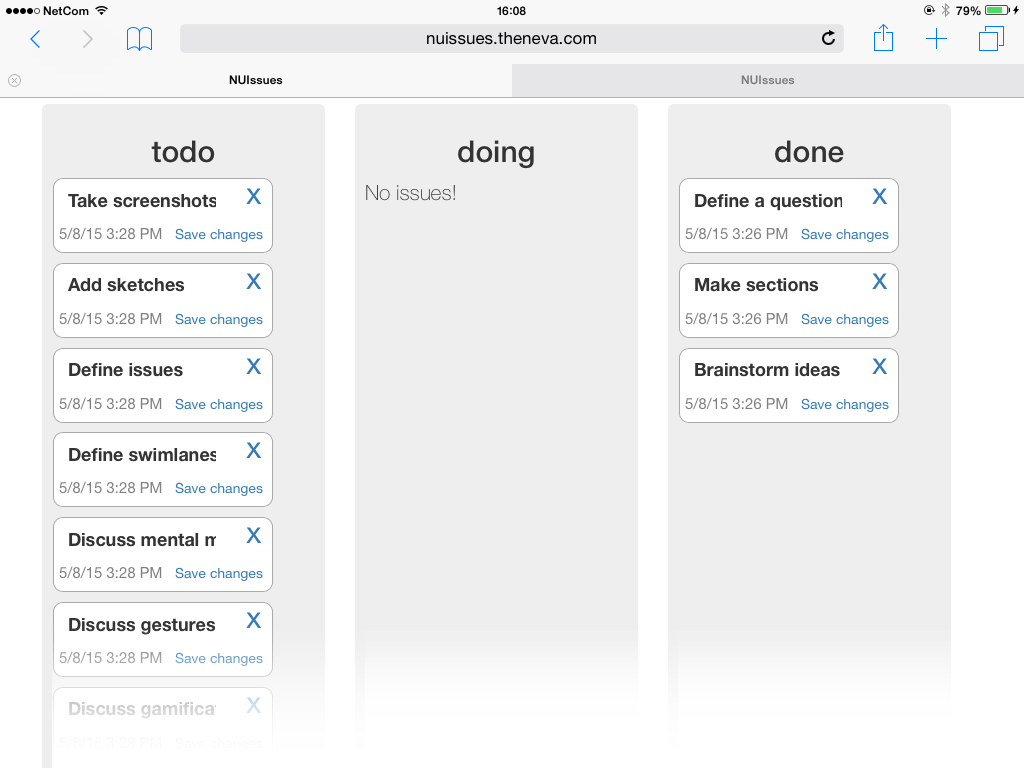
\includegraphics[scale=0.4]{images/nuissues-screenshots/02-default-none-doing}}
    \caption{No issues in the \textit{doing} swimlane}
    \label{figure:meaningful-none-doing}
\end{figure}

Figure \ref{figure:meaningful-none-doing} shows the feedback in response to a swimlane being empty. This hinders confusion with the issues actually being \textit{loaded}, which hinders \textit{apparent} system response times from being an error source by differentiating the two states.

\begin{figure}[H]
    \centerline{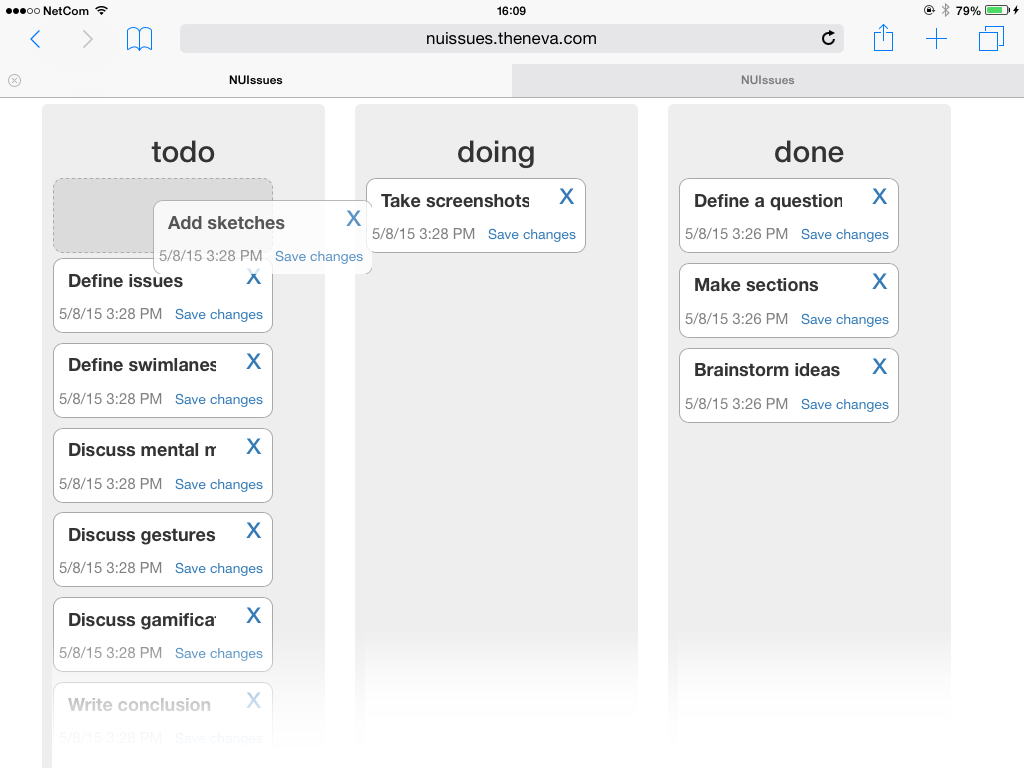
\includegraphics[scale=0.4]{images/nuissues-screenshots/03-dragging-issue}}
    \caption{Card being moved}
    \label{figure:meaningful-card-moving}
\end{figure}

Figure \ref{figure:meaningful-card-moving} shows a card being moved, together with a hint indicating where the issue will land if released. The hinting always finds the closest position and indicates this position. Again, an escape sequence would be very useful here -- but Piaget's property of \textit{negation} is met.

\begin{figure}[H]
    \centerline{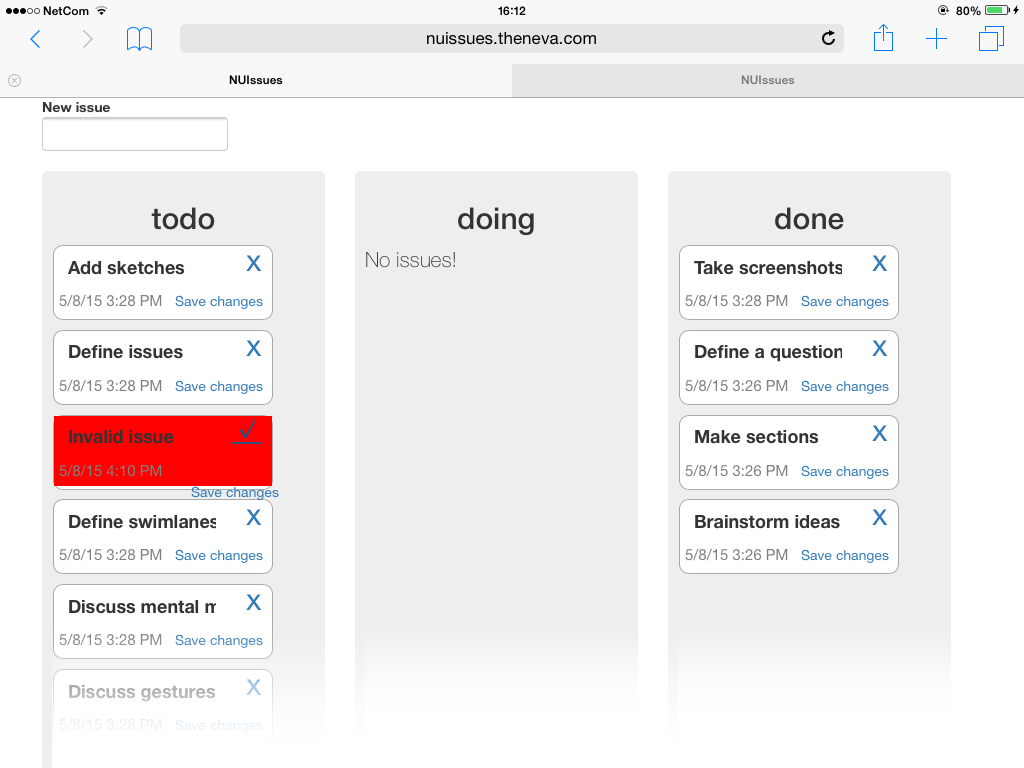
\includegraphics[scale=0.4]{images/nuissues-screenshots/07-invalid-issue-flagged}}
    \caption{Card flagged for deletion}
    \label{figure:meaningful-card-flagged}
\end{figure}

Figure \ref{figure:meaningful-card-flagged} shows a card that is flagged for deletion. The card in its entirety is marked red to indicate to the user that a dangerous action is about to be performed.

\begin{figure}[H]
    \centerline{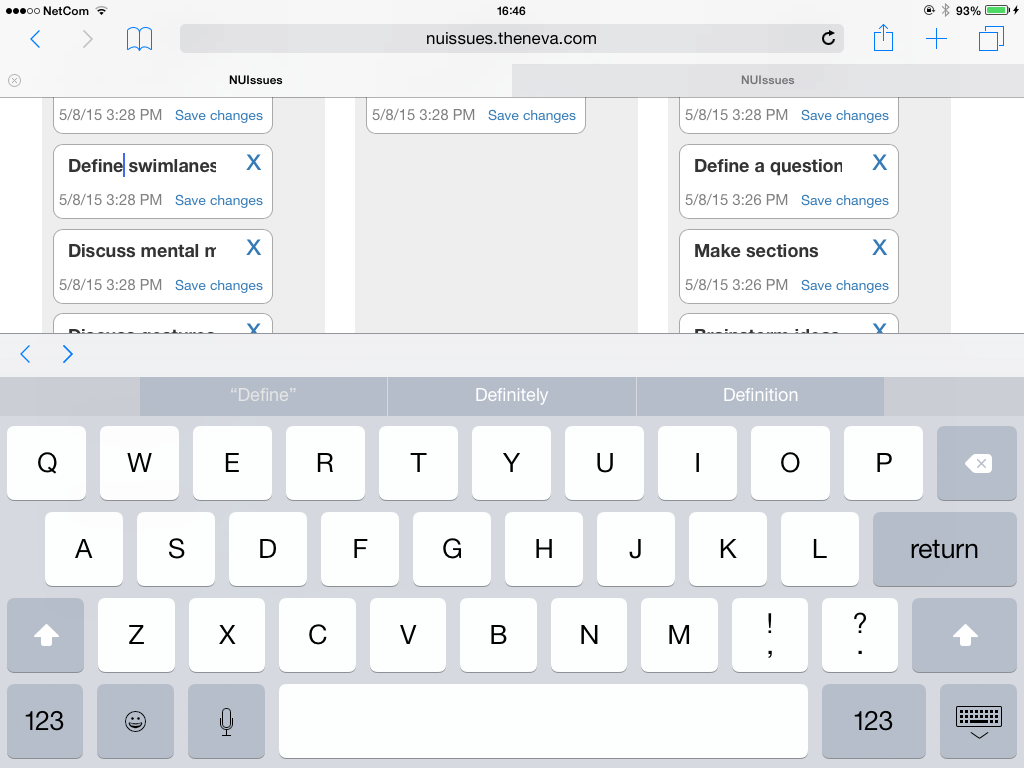
\includegraphics[scale=0.4]{images/nuissues-screenshots/09-editing-issue-title}}
    \caption{Card whose title is being edited}
    \label{figure:meaningful-card-editing}
\end{figure}

Figure \ref{figure:meaningful-card-editing} shows a card whose title is being edited inline. Gray text is used to indicate that it disabled (i.e., not a control), while black text can be interacted with unless it is a heading.

\begin{figure}[H]
    \centerline{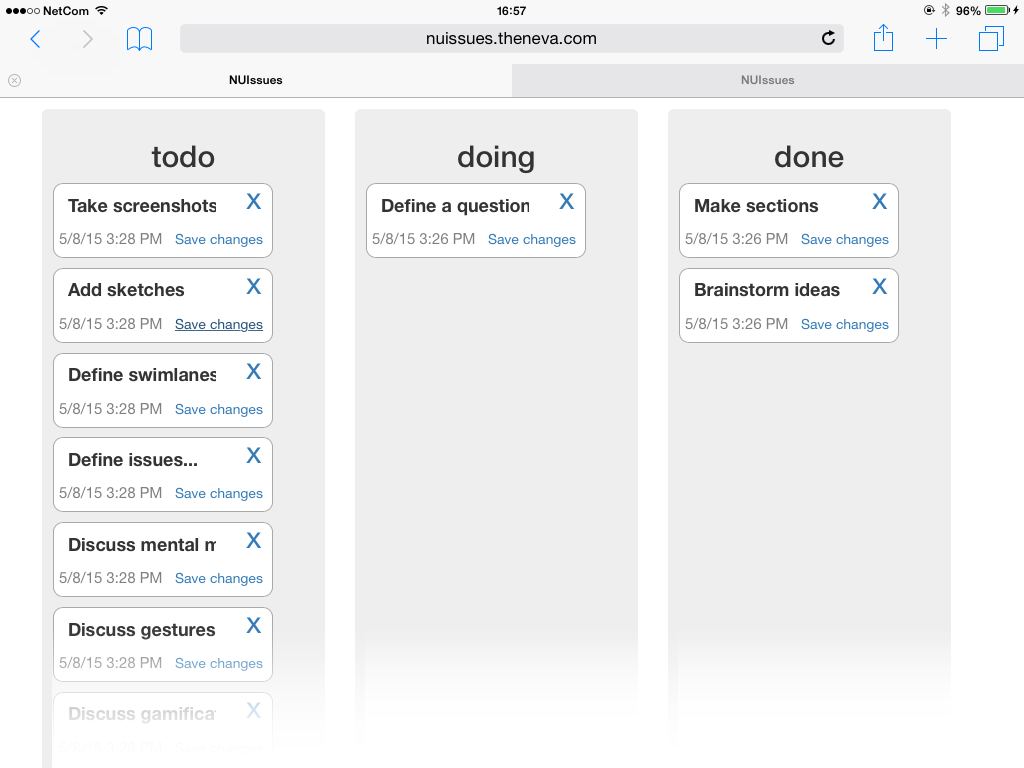
\includegraphics[scale=0.4]{images/nuissues-screenshots/01-default-all-swimlanes}}
    \caption{Default view showing fadeout effect at the bottom of swimlanes}
    \label{figure:meaningful-swimlane-fadeout}
\end{figure}

Figure \ref{figure:meaningful-swimlane-fadeout} demonstrates the fadeout effect at the bottom of each swimlane, which indicates that there is more content to see and that the user can scroll down.

Potential new features can include assigning issues to users, estimating how long tasks will take to complete, and logging work time on each issue.

The application is optimised for touch, but recognising a stylus as an input source would be interesting to for example immediately enter a "sketch attachment" mode where the user can draw a picture which is automatically uploaded to the selected issue.

\subsection{Valuable outcomes}

There are several valuable outcomes from using (a future version of) NUIssues.

\subsubsection{Short-term valuable outcome}

NUIssues in its current state allows anyone to immediately grok the status of the project. If the user wants, they can also update the state of the project in a way that reflects changes for the rest of the team on the move, using a tablet computer.

While some other applications (such as Trello) have mobile applications for managing lists, they generally are not very customisable and lack features like for instance time logging. This should be a priority in a future version of NUIssues.

\subsubsection{Long-term valuable outcome}

Be able to keep track of projects over time (but not across projects), be able to keep a continuous flow of issues % TODO: Talk about archive possibility, statistics

Focus on touch, more tactile approach, bring issues closer by letting people actually interact with them (tangible user interface?) – physical form to digital information (which is really the basis of NUI in the first place, no? – but not really, as there are no real objects; only digital visual representations of the actual work)
